Prototypen består av motorer, kugghjular, sensorer och mikrokontroller. Centralt i det systemet bestämdes att använda Arduino due som ska kommunicera med alla elektriska komponenter.

Anledningen för valet av Arduino due är att den fyller specifikationkraven som ställdes för styrenheten. Utöver dessa finns tillräcklig antal portar för att koppla motorer och sensorer samt att det kan bestämmas farten på hissen som går upp och ner genom PWM signalen. Arduino är en liten plattform, vilken är bra för maskinens begränssad storlek. Tidigare erfanhet att använda och programmera med Arduino samt mögligheten att programmera i C/C++ var också en fördel.

För att kunna kommunicera med användaren används en display som heter 3.2" TFT LCD Touch shield, vilket hjälper användaren att övervaka maskinens tillstånd och eventuella fel.

Figuren~\ref{flodesschma} visar systemets flödesschema.

\begin{figure}[ht]
	\begin{center}
		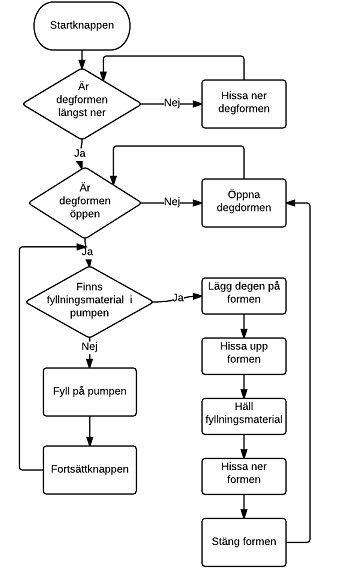
\includegraphics[scale=1.7]{images/Flowchart.png}
		\caption{Systemets flödesschema.}
		\label{flodesschma}	
	\end{center}
\end{figure}